% !TeX program = xelatex
%-------------------------
% Двухстраничное резюме Николая Кукина
%-------------------------

\documentclass[a4paper,10pt]{article}

% ---------- ЯЗЫК И ШРИФТЫ ----------
\usepackage{fontspec}
\usepackage{polyglossia}

\setdefaultlanguage{russian}
\setotherlanguage{english}

\IfFontExistsTF{PT Sans}
    {\setmainfont{PT Sans}}
    {\setmainfont{TeX Gyre Heros}}

% ---------- ОСНОВНЫЕ ПАКЕТЫ ----------
\usepackage[
    a4paper,
    top=1.4cm,
    bottom=1.4cm,
    left=1.5cm,
    right=1.5cm
]{geometry}

\usepackage{graphicx}
\usepackage{enumitem}
\usepackage[hidelinks]{hyperref}
\usepackage{tabularx}
\usepackage{xcolor}
\usepackage{microtype}
\usepackage{fancyhdr}
\usepackage{array}

% ---------- ЦВЕТА ----------
\definecolor{accent}{HTML}{1F4E79}
\definecolor{textgray}{HTML}{4F4F4F}
\definecolor{lightgray}{HTML}{D7DCE2}

% ---------- ОБЩАЯ КОМПОНОВКА ----------
\pagestyle{fancy}
\fancyhf{}
\fancyfoot[C]{%
    \fontsize{8.5}{9.5}\selectfont
    \color{textgray}
    Николай Кукин
    \hspace{5pt}\textbullet\hspace{5pt}
    \thepage
}
\renewcommand{\headrulewidth}{0pt}
\renewcommand{\footrulewidth}{0pt}

\setlength{\parindent}{0pt}
\setlength{\parskip}{0pt}
\setlength{\tabcolsep}{0pt}
\setlength{\emergencystretch}{1em}

\raggedbottom
\raggedright
\urlstyle{same}

% ---------- СПИСКИ ----------
\setlist[itemize]{
    leftmargin=17pt,
    labelsep=6pt,
    itemsep=2.5pt,
    topsep=3pt,
    parsep=0pt,
    partopsep=0pt
}

% ---------- КОМАНДЫ ----------

\newcommand{\resumeSection}[1]{%
    \par
    \vspace{9pt}%
    {\fontsize{14}{16}\selectfont
     \bfseries
     \color{accent}
     #1\par}%
    \vspace{1pt}%
    {\color{accent}\noindent\rule{\textwidth}{0.7pt}\par}%
    \vspace{5pt}%
}

\newcommand{\resumeSubheading}[4]{%
    \begin{tabularx}{\textwidth}{@{}Xr@{}}
        {\fontsize{11}{12.5}\selectfont\bfseries #1}
        &
        {\fontsize{9.7}{11}\selectfont\bfseries #2}
        \\[0.5pt]

        {\fontsize{9.8}{11}\selectfont\itshape #3}
        &
        {\fontsize{9.8}{11}\selectfont\itshape #4}
    \end{tabularx}
    \vspace{2pt}
}

\newcommand{\resumeItem}[1]{%
    \item {\fontsize{9.7}{11.3}\selectfont #1}%
}

\newcommand{\resumeItemListStart}{%
    \begin{itemize}
}

\newcommand{\resumeItemListEnd}{%
    \end{itemize}
}

\newcommand{\tech}[1]{%
    \vspace{1pt}
    {\fontsize{9.5}{10.8}\selectfont
    \textbf{Стек:} #1}%
}

\newcommand{\jobSeparator}{%
    \par
    \vspace{5pt}%
    {\color{lightgray}\noindent\rule{\textwidth}{0.5pt}\par}%
    \vspace{5pt}%
}

\newcommand{\visibleLink}[2]{%
    \href{#1}{\textcolor{accent}{#2}}%
}

% -------------------------------------------
%               ДОКУМЕНТ
% -------------------------------------------

\begin{document}

% =========================================================
% ШАПКА С УВЕЛИЧЕННОЙ ФОТОГРАФИЕЙ
% =========================================================

\begin{tabularx}{\textwidth}{@{}m{4.35cm}@{\hspace{0.8cm}}X@{}}

    % ---------- ФОТО ----------
    \IfFileExists{photo.jpg}{
        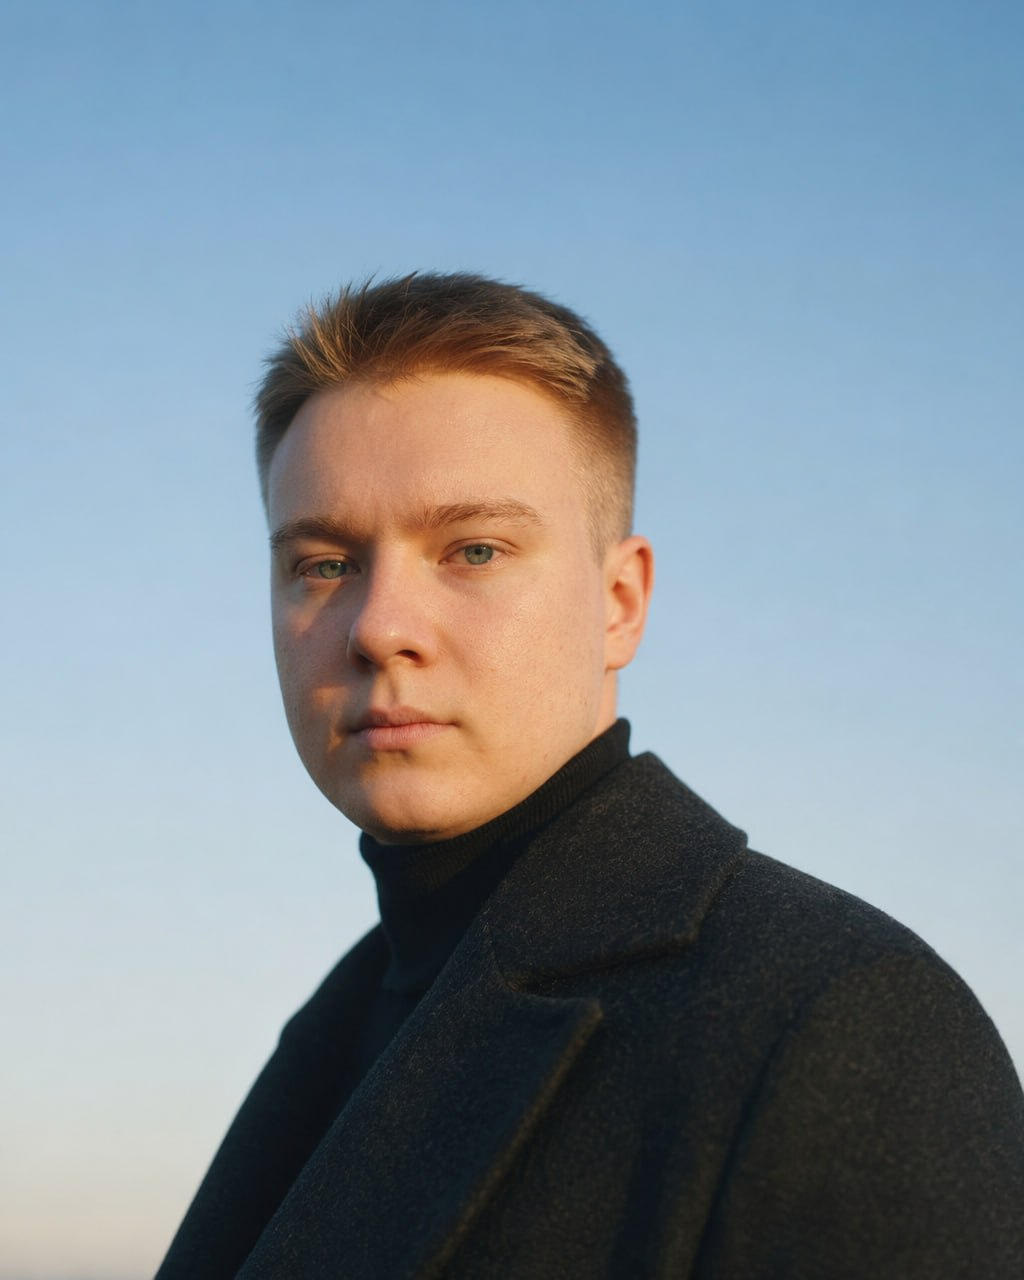
\includegraphics[
            width=4.15cm,
            height=4.85cm,
            keepaspectratio
        ]{photo.jpg}
    }{
        \fbox{
            \parbox[c][4.85cm][c]{4.05cm}{
                \centering
                \color{textgray}
                \fontsize{9}{11}\selectfont
                Добавьте\\
                photo.jpg
            }
        }
    }

    &

    % ---------- ИНФОРМАЦИЯ СПРАВА ----------
    \begin{minipage}[c]{\linewidth}

        {\fontsize{27}{30}\selectfont
        \bfseries Николай Кукин}

        \vspace{4pt}

        {\fontsize{15}{17}\selectfont
        \color{accent}
        \bfseries Backend-разработчик}

        \vspace{12pt}

        {\fontsize{10.5}{12.3}\selectfont
        \href{tel:+79916045191}
        {+7 991 604-51-91}

        \vspace{3.5pt}

        \href{mailto:nikolay.kukin@icloud.com}
        {nikolay.kukin@icloud.com}

        \vspace{3.5pt}

        \href{https://t.me/nikolaykukin}
        {t.me/nikolaykukin}

        \vspace{3.5pt}

        \href{https://github.com/nikolay-kukin}
        {github.com/nikolay-kukin}
        }

    \end{minipage}

\end{tabularx}

\vspace{3pt}

% =========================================================
% ПЕРВАЯ СТРАНИЦА — ТОЛЬКО ОПЫТ
% =========================================================

\resumeSection{Опыт работы}

% ---------- ЛОГИСТИЧЕСКИЙ СТАРТАП ----------
\resumeSubheading
    {Логистический стартап}
    {май 2026 — настоящее время}
    {Fullstack-разработчик}
    {Москва}

{\fontsize{9.8}{11.4}\selectfont
Разработка внутренней системы управления производственными заявками,
складскими и логистическими процессами.
}

\resumeItemListStart

    \resumeItem{
        Разрабатываю REST API и бизнес-логику на Go для процессов
        отгрузки, возвратов, закупок и движения транспорта.
    }

    \resumeItem{
        Реализую сквозные сценарии одновременно в backend,
        мобильном приложении и desktop-dashboard.
    }

    \resumeItem{
        Реализовал идемпотентную обработку транспортных операций,
        серверное хранение статусов автомобилей и корректную доставку
        realtime-уведомлений.
    }

    \resumeItem{
        Участвовал в нормализации legacy-базы: разделении данных
        по схемам, создании справочников и устранении дублирующей логики.
    }

    \resumeItem{
        Разработал редактор BPMN-процессов с версионированием
        и интеграцией с Go API:
        \visibleLink
        {https://github.com/nikolay-kukin/redactor-bpmn}
        {github.com/nikolay-kukin/redactor-bpmn}.
    }

\resumeItemListEnd

\tech{Go, PostgreSQL, REST API, Docker, Flutter, WebSocket}

\jobSeparator

% ---------- ИСТОК ----------
\resumeSubheading
    {НПП «Исток» им. Шокина}
    {август 2024 — настоящее время}
    {Backend-разработчик}
    {Москва}

{\fontsize{9.8}{11.4}\selectfont
Разработка микросервисных B2B-систем на Java для работы с товарными
каталогами, заказами, технической документацией и инженерными проектами.
}

\resumeItemListStart

    \resumeItem{
        Спроектировал систему хранения файлов на базе MinIO и PostgreSQL:
        иерархия каталогов, версионирование, единый API и работа
        с документами, изображениями и техническими материалами.
    }

    \resumeItem{
        Разработал координатор асинхронной ИИ-обработки документов:
        разбиение файлов на страницы, параллельные запросы к ИИ-сервису
        и поэтапное сохранение результатов.
    }

    \resumeItem{
        Реализовал MVP аналитического модуля со сбором событий через Kafka,
        хранением и агрегацией данных в ClickHouse, REST API
        и визуализацией продуктовых метрик:
        \visibleLink
        {https://github.com/nikolay-kukin/analytic-module}
        {github.com/nikolay-kukin/analytic-module}.
    }

    \resumeItem{
        Разработал стенд сравнения HTTP/2 на Spring WebFlux и gRPC,
        провёл нагрузочные тесты и подготовил результаты для выбора
        протокола межсервисного взаимодействия:
        \visibleLink
        {https://github.com/nikolay-kukin/grpc-vs-http2}
        {github.com/nikolay-kukin/grpc-vs-http2}.
    }

    \resumeItem{
        Участвую в проектировании бизнес-логики и API, интеграции сервисов,
        обсуждении архитектуры и выборе технических решений.
    }

\resumeItemListEnd

\tech{
    Java 17, Spring Boot MVC/WebFlux, PostgreSQL, ClickHouse,
    MinIO, Kafka, Docker, Swagger
}

\jobSeparator

% ---------- ВЕБ-КОНСТРУКТОР ----------
\resumeSubheading
    {Индивидуальный проект «Веб-конструктор металлоконструкций»}
    {март 2024 — август 2024}
    {Fullstack-разработчик}
    {Москва}

{\fontsize{9.8}{11.4}\selectfont
Разработал веб-приложение для автоматизации подготовки
технико-коммерческих предложений:
\visibleLink
{https://github.com/nikolay-kukin/chgzabor}
{github.com/nikolay-kukin/chgzabor}.
}

\resumeItemListStart

    \resumeItem{
        Спроектировал микросервисную архитектуру с изолированным
        взаимодействием сервисов внутри Docker-сети.
    }

    \resumeItem{
        Реализовал расширяемый модуль расчёта конструкций с возможностью
        добавлять новые типы изделий без изменения существующей логики.
    }

    \resumeItem{
        Разработал генератор PDF-документов на Apache PDFBox
        и браузерный интерфейс настройки изделия.
    }

    \resumeItem{
        Сократил время подготовки технико-коммерческого предложения
        с нескольких дней до нескольких минут.
    }

\resumeItemListEnd

\tech{
    Java 17, Spring Boot, Apache PDFBox, Docker,
    HTML, CSS, JavaScript
}

% =========================================================
% ВТОРАЯ СТРАНИЦА
% =========================================================

\newpage

% ---------- О СЕБЕ ----------
\resumeSection{О себе}

{\fontsize{10}{11.8}\selectfont
Backend-разработчик с коммерческим опытом создания B2B-систем,
внутренних производственных сервисов и микросервисных приложений.
Основной стек — Java, Spring Boot и PostgreSQL; также разрабатываю
backend на Go и сквозные сценарии с Flutter-клиентами. Участвую
в проектировании архитектуры, API, бизнес-логики и моделей данных.
Использую ИИ-инструменты для анализа, разработки и автоматизации
рутинных задач.
}

% ---------- ОБРАЗОВАНИЕ ----------
\resumeSection{Образование}

\begin{tabularx}{\textwidth}{@{}Xr@{}}

    {\fontsize{11}{12.5}\selectfont\bfseries
    РТУ МИРЭА}

    &

    {\fontsize{9.8}{11}\selectfont\bfseries
    2022–2026}

    \\[2pt]

    \multicolumn{2}{@{}l@{}}{
        \fontsize{10}{11.6}\selectfont
        \textbf{Бакалавриат с отличием —
        «Информатика и вычислительная техника»}
    }

    \\[2pt]

    \multicolumn{2}{@{}p{\textwidth}@{}}{
        \fontsize{9.8}{11.4}\selectfont
        Автоматизация и цифровизация производств
        радиоэлектронной промышленности
    }

\end{tabularx}

\vspace{8pt}

\begin{tabularx}{\textwidth}{@{}Xr@{}}

    {\fontsize{10.5}{12}\selectfont\bfseries
    Профессиональная переподготовка}

    &

    {\fontsize{9.8}{11}\selectfont\bfseries
    2026}

    \\[2pt]

    \multicolumn{2}{@{}l@{}}{
        \fontsize{9.8}{11.4}\selectfont
        РТУ МИРЭА — Менеджер по информационным технологиям
    }

\end{tabularx}

\vspace{7pt}

\begin{tabularx}{\textwidth}{@{}Xr@{}}

    {\fontsize{10.5}{12}\selectfont\bfseries
    Профессиональная переподготовка}

    &

    {\fontsize{9.8}{11}\selectfont\bfseries
    2026}

    \\[2pt]

    \multicolumn{2}{@{}l@{}}{
        \fontsize{9.8}{11.4}\selectfont
        РТУ МИРЭА — Технологии DevOps
    }

\end{tabularx}

% ---------- ТЕХНИЧЕСКИЕ НАВЫКИ ----------
\resumeSection{Технические навыки}

{\fontsize{10}{11.8}\selectfont

\textbf{\color{accent}Основные}

\vspace{3pt}

Java 17, Spring Boot MVC/WebFlux, PostgreSQL, MinIO, Docker, Swagger

\vspace{9pt}

\textbf{\color{accent}Дополнительные}

\vspace{3pt}

Go, Apache Kafka, ClickHouse, Redis, REST API, WebSocket, Apache PDFBox

\vspace{9pt}

\textbf{\color{accent}Базовый уровень}

\vspace{3pt}

React, JavaScript, HTML, CSS, Dart, Flutter

}

% ---------- ДОПОЛНИТЕЛЬНОЕ ОБУЧЕНИЕ ----------
\resumeSection{Дополнительное обучение}

{\fontsize{10}{11.8}\selectfont
Проходил дополнительное обучение по Java, тестированию информационных
систем, алгоритмам, ИИ, промтингу и разработке AI-агентов. Участвовал
в интенсивах и тренировках Яндекса, а также выступал с докладом
на студенческой конференции РТУ МИРЭА.
}

% ---------- ЯЗЫКИ ----------
\resumeSection{Языки}

{\fontsize{10}{11.8}\selectfont
\textbf{Русский} — родной
\hspace{15pt}
\textbullet
\hspace{15pt}
\textbf{Английский} — A1, начальный уровень
}

% ---------- СЕРТИФИКАТЫ ----------
\resumeSection{Сертификаты и дипломы}

{\fontsize{10}{11.8}\selectfont
Имею сертификаты по Java, тестированию, алгоритмам и применению
ИИ-инструментов, а также дипломы о высшем образовании и двух программах
профессиональной переподготовки. Все подтверждающие документы доступны
по ссылке: \visibleLink
{https://disk.yandex.ru/d/uQvg0pOUF47oiA}
{disk.yandex.ru/d/uQvg0pOUF47oiA}
}

\end{document}